<<<<<<< HEAD
For the purpose of this study, we generated three variations on a “Battle Asteroids” game. In each of these variations, players are made to control a ship and compete against an AI-controlled player. The player is able to control the rotation of the ship, apply thrust, and fire a finite-number of missiles. If the player travels off the side of the screen, they re-appear on the opposite side of the map. A number of pickups are distributed around the map, and any player that “collects” the pickup scores a number of points. In all of the variations, the player is also able to score points by shooting the opposing ship. The game ends after a set amount of time, with the ship with the most points being classed as the winner.
=======
For the purpose of this study, we generated three variations of a “Battle Asteroids” game. In each of these variations, players are made to control a ship and compete against an AI-controlled player. The player is able to control the rotation of the ship, apply thrust, and fire a finite number of missiles. If the player travels off the side of the screen, they re-appear on the opposite side of the map. A number of pickups are distributed around the map, and any player that “collects” the pickup scores a number of points. In all of the variations, the player is also able to score points by shooting the opposing ship. The game ends after a set amount of time, with the ship with the most points being classed as the winner.
>>>>>>> 3a3d8159e193104eced80ebd80931f7bec344b89

The first variation of the base game was the inclusion of simple asteroids. These asteroids are distributed randomly at the start of the game, and are destroyed when they are shot or and ship collides with them. Players are given no explicit reward for shooting asteroids, and have their score penalised for colliding with the asteroids. The second variation used also included asteroids, but split rather than get destroyed when they collide with missiles or ships.

<<<<<<< HEAD
The intention of these variants was twofold; firstly, we hoped that the inclusion of asteroids would force the players to move around the map more, and secondly we hoped that by introducing additional complexity to the game it would be easier to distinguish between “good” and “bad” players.

\begin{figure}
	\caption{Screenshots from the three game modes.}
	\begin{subfigure}[b]{0.15\textwidth}
		\center
		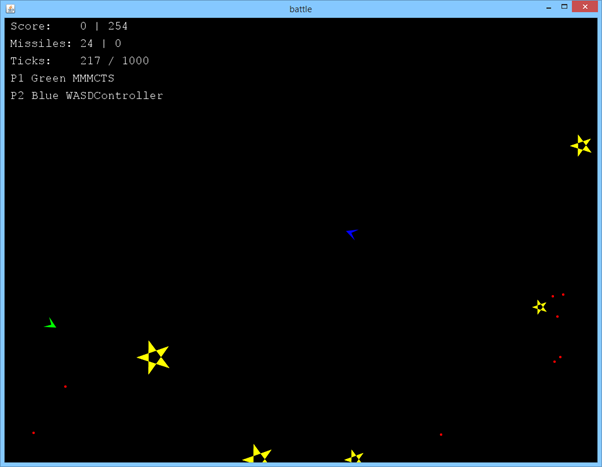
\includegraphics[scale=0.17]{resources/gamemode2}
		\caption{Without asteroids\\\hspace{\textwidth}}
	\end{subfigure}
	\begin{subfigure}[b]{0.15\textwidth}
		\center
		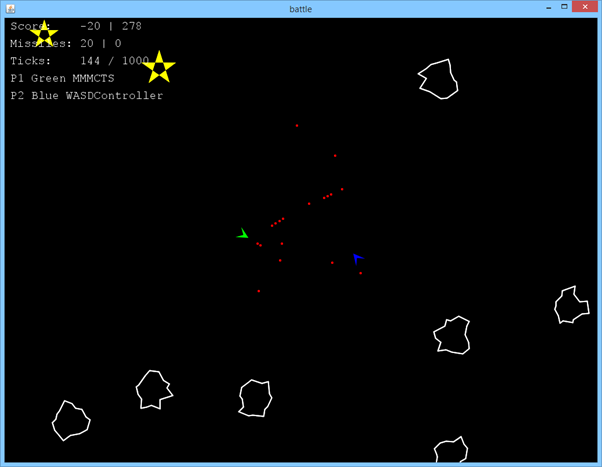
\includegraphics[scale=0.17]{resources/gamemode1}
		\caption{With simple\\asteroids}
	\end{subfigure}
	\begin{subfigure}[b]{0.15\textwidth}
		\center
		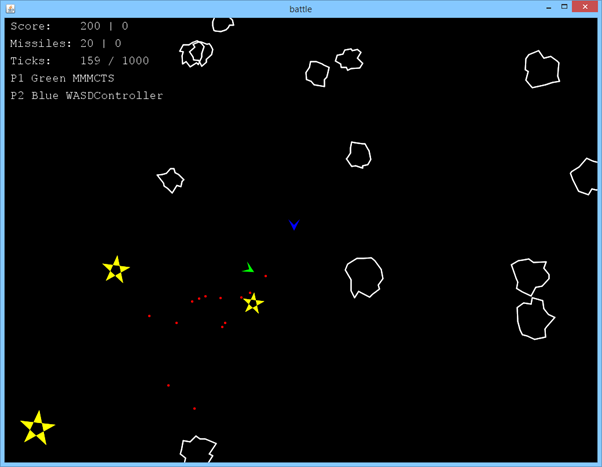
\includegraphics[scale=0.17]{resources/gamemode0}
		\caption{With splitting\\asteroids}
	\end{subfigure}
\end{figure}
	
=======
The intention behind the creation of these variants was twofold; firstly, we hoped that the inclusion of asteroids would force the players to move around the map more, and secondly we hoped that by introducing additional complexity to the game it would be easier to distinguish between “good” and “bad” players.
>>>>>>> 3a3d8159e193104eced80ebd80931f7bec344b89
